
%\documentclass[manuscript]{acmart}
%\documentclass[acmsmall]{acmart}
%\settopmatter{printacmref=false}


\documentclass[
  a4paper,
  12pt,
  DIV=12,        % höherer Wert = schmalere Ränder, weniger Whitespacmi
  parskip=half,  % Absätze mit halbem Abstand statt Einzug
  headings=small % kleinere Überschriften, weniger vertikaler Abstand
]{scrartcl}

%\documentclass[a4paper,11pt]{scrartcl}
%\documentclass[a4paper,11pt]{report}
%\documentclass[a4paper,12pt]{book}
\usepackage[utf8]{inputenc}
\usepackage[german]{babel}
\usepackage[T1]{fontenc}
\usepackage{lmodern}
\usepackage[inkscapelatex=false]{svg}
% Texte im SVG von Inkscape setzen lassen, nicht durch die Dokumentschrift ersetzen
\svgsetup{inkscapelatex=false}
\usepackage{amsmath}
\usepackage{caption}
\usepackage{gensymb}
\usepackage{microtype}
\usepackage{longtable}
\usepackage{tabularx}   % Spalten, die die restliche Zeilenbreite auffüllen (X-Spalte)
\usepackage{booktabs}   % \toprule \midrule \bottomrule (in mobrob_table.tex verwendet)
\usepackage{wrapfig}    % Textumfluss um Abbildungen
\usepackage{array}
\usepackage{calc}

\usepackage[citecolor=black, colorlinks=true, linkcolor=black, urlcolor=blue]{hyperref}


%\usepackage{geometry}
\usepackage{siunitx}
%\geometry{margin=2.5cm}


\usepackage{amsthm}
\usepackage{mdframed}
\usepackage{enumitem}

\newmdtheoremenv{theorem}{Theorem}

\theoremstyle{definition}
\newmdtheoremenv{derivation}{Derivation}

\providecommand{\tightlist}{%
  \setlength{\itemsep}{0pt}\setlength{\parskip}{0pt}}

%\mdfdefinestyle{leftline}{
%    topline=false, bottomline=false, rightline=false,
%    linewidth=2pt, linecolor=gray
%}
\theoremstyle{definition}
\newmdtheoremenv[style=leftline]{myalgorithm}{Algorithm}




%\usepackage{fancyvrb}







\let\Bbbk\relax
\usepackage{amssymb}


\usepackage{yfonts}

\usepackage{kvmap}

\usepackage[
    backend=biber,
    style=alphabetic,
    sortlocale=de_DE,
    natbib=true,
    %url=false,
    doi=true,
    %eprint=false
]{biblatex}
% \addbibresource{Literaturrecherche-Stefan-Etringer/algo-references.bib}

%\usepackage[
%    backend=biber,
%    style=alphabetic,
%    sortlocale=de_DE,
%    natbib=true,
%    %url=false,
%    doi=true,
%    %eprint=false
%]{biblatex}
%\addbibresource{Literaturrecherche-Dennis/mobrob_references.bib}

\usepackage[autostyle=true,german=quotes]{csquotes}
\usepackage{trfsigns} %fourier transform arrow
\usepackage{mathrsfs} %fourier F
\usepackage{commath}

\usepackage{pgfplots}
\pgfplotsset{compat=1.18}

\usepackage{xcolor}
\usepackage{listings}
\usepackage[european]{circuitikz}
\ctikzset{tripoles/european not symbol=ieee circle}

%\usepackage[shading]{moeptikz}
%\moeptikzset{shading=true}

%\usepackage{german,longtable}

\usepackage{xcolor}
\usepackage{color}
\usepackage{url}

\usepackage{xfrac}

\usepackage{listings}
\usepackage{verbatimbox}

\usepackage{algorithm}
\usepackage{algpseudocode}

\usepackage{multirow}
\usepackage{float}
\usepackage{pdflscape}   % einzelne Querformatseiten (im PDF gedreht)

%%%% TIKZ

\usepackage{tikz}

\usepackage{pgfplots}
\usetikzlibrary{calc,
trees,positioning,arrows,
chains,shapes.geometric,
decorations.pathreplacing,
decorations.pathmorphing,shapes,
matrix,shapes.symbols,
plotmarks}
%\tikzexternalize[prefix=figures/]

%\tikzset{%
%  block/.style    = {draw, thick, rectangle, minimum height = 3em,
%    minimum width = 3em},
%  sum/.style      = {draw, circle, node distance = 2cm}, % Adder
%  input/.style    = {coordinate}, % Input
%  output/.style   = {coordinate} % Output
%}
% Defining string as labels of certain blocks.
%\newcommand{\suma}{\Large$+$}
%\newcommand{\multa}{\Large$\times$}
%\newcommand{\inte}{$\displaystyle \int$}
%\newcommand{\derv}{\huge$\frac{d}{dt}$}

\usetikzlibrary{arrows,automata,positioning}
%\usepackage{automata}


%%% END TIKZ

\usepackage[section]{placeins}

\usepackage{textcomp}


\usepackage{listings}
\usepackage{verbatimbox}

\usepackage{bold-extra}

\usepackage{framed}

%\usepackage{fancyhdr}
%\pagestyle{fancy}
%\lhead{\leftmark}
%\chead{}
%\rhead{}
%\lfoot{}
%\cfoot{\thepage}
%\rfoot{}
%\renewcommand{\headrulewidth}{0.2pt}
%\renewcommand{\footrulewidth}{0.2pt}



\newcommand{\Z}{\mathbb{Z}}
\newcommand{\R}{\mathbb{R}}
\newcommand{\C}{\mathbb{C}}
\newcommand{\N}{\mathbb{N}}
\newcommand{\SqrtNy}{$\sqrt{\textsc{Ny}}$}
\newcommand{\conj}{\overline}
\newcommand{\Kset}{\textswab{K}}
\newcommand{\Qset}{\textswab{Q}}
\newcommand{\ceil}[1]{\left\lceil #1 \right\rceil}
\newcommand{\floor}[1]{\left\lfloor #1 \right\rfloor}
\newcommand{\sorted}[1]{\textsc{sort}\left\lbrace #1 \right\rbrace}
\newcommand{\SNRgain}{a_{SNR}}
\newcommand{\EQgain}{a_{EQ}}
\newcommand{\SIRgain}{a_{SIR}}
\newcommand{\SNIRgain}{a_{SINR}}
\newcommand{\SNR}{\textsc{SNR}}
\newcommand{\CIRgain}{a_{CIR}}
\newcommand{\CINRgain}{a_{CINR}}
\newcommand{\CNR}{\textsc{CNR}}
\newcommand{\CINR}{\textsc{CINR}}
\newcommand{\HPAModel}{ Hughes 1177H TWTA }
\newcommand{\bigO}{\mathcal{O}}
\newcommand{\CopWinCompl}{2.375377}
\newcommand{\IBO}{\textsc{IBO}}
\newcommand{\OBO}{\textsc{OBO}}
\newcommand{\spacepage}{\newpage\null\thispagestyle{empty}\newpage}
\newcommand{\satcom}{ SatCom }
\newcommand{\db}{~\text{dB}}


\definecolor{mGreen}{rgb}{0,0.6,0}
\definecolor{mGray}{rgb}{0.5,0.5,0.5}
\definecolor{mPurple}{rgb}{0.58,0,0.82}
\definecolor{backgroundColour}{rgb}{0.95,0.95,0.92}

\lstdefinestyle{CStyle}{
    backgroundcolor=\color{backgroundColour},
    commentstyle=\color{mGreen},
    keywordstyle=\color{magenta},
    numberstyle=\tiny\color{mGray},
    stringstyle=\color{mPurple},
    basicstyle=\footnotesize,
    breakatwhitespace=false,
    breaklines=true,
    captionpos=b,
    keepspaces=true,
    numbers=left,
    numbersep=5pt,
    showspaces=false,
    showstringspaces=false,
    showtabs=false,
    tabsize=2,
    language=C
}

\lstdefinelanguage{VHDL}{
  morekeywords=[1]{library,use,all,entity,is,port,in,out,end,architecture,of,begin,process,if,then,else,elsif,when,others,signal,variable,wait,for,loop},
  morecomment=[l]--,
  morestring=[b]",
  sensitive=true
}

\lstset{
  language=VHDL,
  basicstyle=\ttfamily\small,
  keywordstyle=\color{blue},
  commentstyle=\color{gray},
  stringstyle=\color{red},
  numbers=left,
  numberstyle=\tiny,
  stepnumber=1,
  numbersep=8pt,
  frame=single,
  breaklines=true,
  captionpos=b
}

\lstset{numbers=none}

%\newcounter{example}
%\renewcommand{\theexample}{\thesection.\arabic{example}}


% Default fixed font does not support bold face
\DeclareFixedFont{\ttb}{T1}{txtt}{bx}{n}{12} % for bold
\DeclareFixedFont{\ttm}{T1}{txtt}{m}{n}{12}  % for normal

% Custom colors
\usepackage{color}
\definecolor{deepblue}{rgb}{0,0,0.5}
\definecolor{deepred}{rgb}{0.6,0,0}
\definecolor{deepgreen}{rgb}{0,0.5,0}

\usepackage{listings}

% Python style for highlighting
\newcommand\pythonstyle{\lstset{
language=Python,
basicstyle=\ttm,
morekeywords={self},              % Add keywords here
keywordstyle=\ttb\color{deepblue},
emph={MyClass,__init__},          % Custom highlighting
emphstyle=\ttb\color{deepred},    % Custom highlighting style
stringstyle=\color{deepgreen},
frame=tb,                         % Any extra options here
showstringspaces=false
}}


% Python environment
\lstnewenvironment{python}[1][]
{
\pythonstyle
\lstset{#1}
}
{}

% Python for external files
\newcommand\pythonexternal[2][]{{
\pythonstyle
\lstinputlisting[#1]{#2}}}

% Python for inline
\newcommand\pythoninline[1]{{\pythonstyle\lstinline!#1!}}





\nocite{*}


\begin{document}
%\pagenumbering{roman}



\title{Coasterbot}
\subtitle{Alternativenbeschreibung}
\author{Stefan Etringer}
%\email{gereonsuch@suchdsp.com}
%\affiliation{
%  \institution{Wilhelm Büchner University of Applied Sciences}
%  \department{Computer Engineering}
%  \city{Hof}
%  \country{Germany}
%}



\begin{titlepage}
  \begin{center}
    {\large Wilhelm Büchner University of Applied Sciences} \\[0.3em]

    {\normalsize Projektseminar Master}
\vspace{5em}

    {\LARGE\bfseries Coasterbot} \\[0.5em]

    {\large Alternativenbeschreibung} \\[1em]

    {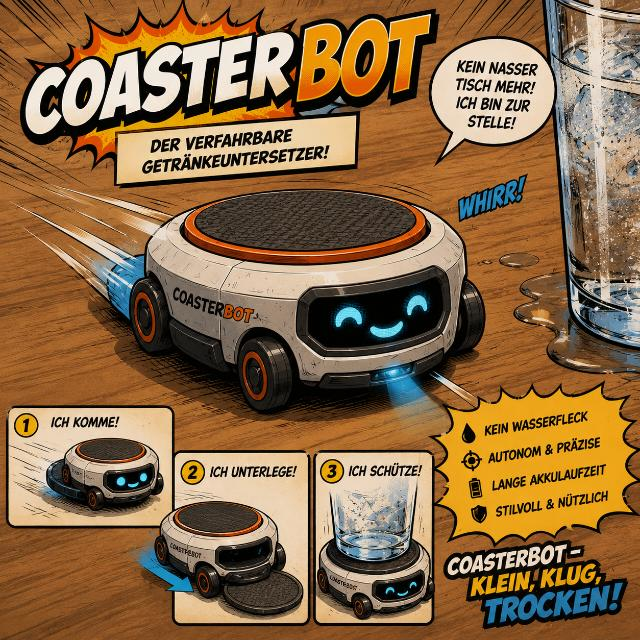
\includegraphics[width=0.38\textwidth]{coasterbot.png}} \\[1em]

\vspace{4em}

    {\normalsize
\begin{tabular}{ll}
Dennis Borutta, B. Eng & dennis.borutta@outlook.com\\
Stefan Etringer, B. Eng & mail@stefan.works\\
Gereon Such, M. Sc. & gereonsuch@gmail.com\\
\end{tabular}
    }
  \end{center}


\end{titlepage}


% einleitung preambel etc.


% Versionshistorie des Dokuments -- eigene Seite direkt nach dem Titelblatt
\section*{Versionshistorie}

\begin{tabularx}{\textwidth}{@{}clp{2.6cm}X@{}}
\toprule
\textbf{Version} & \textbf{Datum} & \textbf{Bearbeiter} & \textbf{Änderungen}\\
\midrule
1 & 17.08.2026 & Etringer & Erstfassung der Alternativenbeschreibung\\
2 & 17.08.2026 & Borutta & Detaillierung Kapitel Mechanik\\
3 & 17.08.2026 & Such & Sensorik Ergänzungen\\
\bottomrule
\end{tabularx}


\newpage

\tableofcontents

\newpage

\section{Alternativenbeschreibung}\label{alternativenbeschreibung}

\subsection{Ziel und Vorgehensweise}\label{ziel-und-vorgehensweise}

Im Rahmen der Projektarbeit „Coasterbot -- Entwicklung eines Prototyps``
wird ein handtellergroßer Roboter entwickelt, der sich selbstständig auf
einem Tisch bewegen, Getränkeuntersetzer gezielt ausgeben und diese
anschließend automatisiert wieder aufnehmen kann.

Für die Umsetzung des Prototyps bestehen für verschiedene Teilbereiche
unterschiedliche technische Lösungsansätze. Im Rahmen der
Alternativenbetrachtung werden diese Ansätze gegenübergestellt und
hinsichtlich ihrer Eignung für das Projekt bewertet.

Die Betrachtung orientiert sich dabei an den funktionalen und
technischen Anforderungen des Coasterbots. Berücksichtigt werden
insbesondere die Bereiche Software bzw. Algorithmen, Recheneinheit,
Sensorik, Aktorik, Energieversorgung und Mechanik.

Für jede betrachtete Funktion werden zunächst die zugrunde liegende
Herausforderung und die mögliche Lösungsvariante beschrieben.
Anschließend werden geeignete Alternativen aufgezeigt und hinsichtlich
ihrer jeweiligen Vor- und Nachteile gegenübergestellt. Die letztendliche
Auswahl einer Variante erfolgt unter Berücksichtigung der Anforderungen
des Projekts, der Komplexität der Umsetzung sowie der Eignung für einen
funktionsfähigen Prototyp.

\section{Systemarchitektur}\label{systemarchitektur}

Die Systemarchitektur des Coasterbots lässt sich grundsätzlich in die
Bereiche Elektrik und Energieversorgung, Algorithmen und Mechanik
unterteilen.

Auf Softwareseite umfasst das System vor allem die Recheneinheit sowie
Algorithmen zur Navigation und Manipulationsplanung. Die Hardware
umfasst unter anderem Sensorik zur Hindernis- und Tischkantenerkennung,
Komponenten zur Positionsbestimmung, Antriebsmotoren sowie die Mechanik
zur Aufnahme und Ablage der Untersetzer.

Eine mögliche Systemarchitektur sieht die Kombination einer
Recheneinheit mit geeigneter Sensorik und Motorsteuerung vor. Die
Auswahl der konkreten Komponenten und Verfahren wird in den folgenden
Abschnitten anhand der jeweiligen Teilfunktionen betrachtet.

\section{Algorithmen}\label{algorithmen}

\subsection{Globale Fahrwegplanung}\label{globale-fahrwegplanung}

\subsubsection{Herausforderung}\label{herausforderung}

Der Coasterbot muss eine Zielposition auf dem Tisch erreichen. Dabei
soll ausgehend von der aktuellen Position ein geeigneter globaler
Fahrweg bestimmt werden. Als Grundlage kann dabei eine bekannte
Tischkarte dienen.

\subsubsection{Mögliche Lösung: A*}\label{muxf6gliche-luxf6sung-a}

Für die heuristische globale Pfadplanung kann der A\emph{-Algorithmus
eingesetzt werden. A} verbindet die bisher angefallenen Kosten eines
Pfades mit einer Heuristik zur Abschätzung der noch verbleibenden
Kosten. Dadurch kann gegenüber einer rein ungerichteten Suche gezielt
ein geeigneter Weg zum Ziel bestimmt werden.

\subsubsection{Alternativen}\label{alternativen}

\textbf{Dijkstra-Algorithmus}

Dijkstra stellt eine Alternative zur globalen Pfadplanung dar. Der
Algorithmus bestimmt kürzeste Wege in einem gewichteten Graphen und kann
als Referenz für eine optimale Pfadplanung dienen. Im Vergleich zu A*
wird jedoch keine zielgerichtete Heuristik verwendet.

\textbf{Breitensuche (BFS)}

Die Breitensuche kann für ungewichtete Graphen eingesetzt werden. Sie
ist konzeptionell einfach und eignet sich insbesondere dann, wenn alle
Bewegungen dieselben Kosten besitzen.

\subsubsection{Bewertung}\label{bewertung}

Für den Coasterbot ist zu bewerten, wie effizient der Algorithmus einen
Weg zur Zielposition bestimmen kann und welche Anforderungen an die
zugrunde liegende Karte gestellt werden.

Die Auswahl zwischen A*, Dijkstra und BFS erfolgt daher anhand der
Eigenschaften der Tischkarte, der Gewichtung der Bewegungen und der
Anforderungen an die Effizienz der Pfadplanung.

\subsection{Lokale
Kollisionsvermeidung}\label{lokale-kollisionsvermeidung}

\subsubsection{Herausforderung}\label{herausforderung-1}

Während der Fahrt können Hindernisse wie Gläser, Teller oder Personen
den ursprünglich geplanten Fahrweg blockieren. Der Roboter muss daher
kurzfristig auf Veränderungen seiner direkten Umgebung reagieren können.

\subsubsection{Mögliche Lösung: Dynamic Window Approach
(DWA)}\label{muxf6gliche-luxf6sung-dynamic-window-approach-dwa}

Der Dynamic Window Approach berücksichtigt die Bewegungsdynamik des
Roboters und ermöglicht eine lokale Reaktion auf Hindernisse. Dadurch
kann der Roboter auf kurzfristige Veränderungen der Umgebung reagieren,
ohne den globalen Fahrweg vollständig neu berechnen zu müssen.

\subsubsection{Alternativen}\label{alternativen-1}

\textbf{Potentialfelder}

Bei der Methode der Potentialfelder wird das Ziel als anziehendes und
Hindernisse als abstoßendes Potential modelliert. Die Methode ist
vergleichsweise einfach, kann jedoch lokale Minima aufweisen.

\textbf{Adaptive bzw. neuronale DWA}

Eine Erweiterung des DWA-Ansatzes kann insbesondere bei dynamischen
Hindernissen eingesetzt werden. Dabei kann die lokale Fahrplanung an
veränderte Umgebungsbedingungen angepasst werden.

\subsubsection{Bewertung}\label{bewertung-1}

Bei der Auswahl sind die Reaktionsfähigkeit gegenüber Hindernissen, die
Komplexität der Implementierung sowie das Verhalten bei dynamischen
Hindernissen zu berücksichtigen.

\subsection{Dynamische Fahrplanung}\label{dynamische-fahrplanung}

\subsubsection{Herausforderung}\label{herausforderung-2}

Verändert sich die Umgebung während der Fahrt wiederholt, kann der
ursprünglich berechnete globale Fahrweg ungültig werden. Der Roboter
benötigt daher ein Verfahren, mit dem Änderungen der Umgebung bei der
Pfadplanung berücksichtigt werden können.

\subsubsection{Mögliche Lösung: D*
Lite}\label{muxf6gliche-luxf6sung-d-lite}

D* Lite ermöglicht eine inkrementelle Neuberechnung eines Pfades.
Anstatt bei jeder Veränderung die gesamte Planung von Grund auf neu
durchzuführen, können Änderungen gezielt in die bestehende Planung
einbezogen werden.

\subsubsection{Alternativen}\label{alternativen-2}

\textbf{D}*

D* stellt einen alternativen Ansatz für die dynamische Pfadplanung dar
und wurde ebenfalls für Umgebungen entwickelt, in denen sich die
verfügbaren Wege verändern können.

\textbf{LPA}*

LPA* (Lifelong Planning A*) stellt einen weiteren inkrementellen Ansatz
zur Pfadplanung dar. Der Algorithmus ist insbesondere für Situationen
geeignet, in denen wiederholt Änderungen am zugrunde liegenden Graphen
auftreten.

\subsubsection{Bewertung}\label{bewertung-2}

Die Verfahren unterscheiden sich hinsichtlich ihrer Vorgehensweise bei
der inkrementellen Neuberechnung und ihrer Eignung für wiederholte
Änderungen der Umgebung.

Für den Coasterbot ist zu prüfen, welches Verfahren bei den erwarteten
Veränderungen der Tischumgebung ein angemessenes Verhältnis zwischen
Planungsaufwand und Reaktionsfähigkeit bietet.

\subsection{Manipulationsplanung}\label{manipulationsplanung}

\subsubsection{Herausforderung}\label{herausforderung-3}

Der Coasterbot muss Getränkeuntersetzer aufnehmen und gezielt wieder
ablegen können. Dabei muss sowohl die gewünschte Greif- bzw.
Aufnahmeposition als auch die spätere Ablageposition berücksichtigt
werden.

\subsubsection{Mögliche Lösung: Inverse Kinematik und
RRT*}\label{muxf6gliche-luxf6sung-inverse-kinematik-und-rrt}

Eine mögliche Lösung besteht in der Kombination aus inverser Kinematik
und RRT\emph{. Die inverse Kinematik kann dazu verwendet werden, aus
einer gewünschten Zielpose geeignete Gelenkstellungen abzuleiten. RRT}
kann anschließend für eine kollisionsfreie Bewegungsplanung eingesetzt
werden.

\subsubsection{Alternativen}\label{alternativen-3}

\textbf{Roboter mit Sauger}

Die Aufnahme des Untersetzers kann alternativ über einen Sauger
erfolgen. Dabei wird der Untersetzer durch eine entsprechende
Saugvorrichtung aufgenommen und anschließend an der gewünschten Position
abgelegt.

\textbf{Roboter mit Greifer}

Eine weitere Möglichkeit ist die Verwendung eines mechanischen Greifers.
Dieser kann den Untersetzer greifen und kontrolliert bewegen.

\textbf{Manuelle Einlage}

Als einfachste Alternative kann der Untersetzer manuell in eine dafür
vorgesehene Aufnahme des Roboters eingelegt werden.

\textbf{Magnetischer Heber}

Falls geeignete magnetische Untersetzer verwendet werden, kann
alternativ ein magnetischer Heber eingesetzt werden.

\subsubsection{Bewertung}\label{bewertung-3}

Die Varianten unterscheiden sich hinsichtlich mechanischer Komplexität,
Zuverlässigkeit bei der Aufnahme und Ablage sowie der Anforderungen an
die Steuerung.

\subsection{Lokalisierung}\label{lokalisierung}

\subsubsection{Herausforderung}\label{herausforderung-4}

Damit der Coasterbot seine Fahrbewegung planen und ausführen kann, muss
seine aktuelle Position beziehungsweise Orientierung bestimmt werden.

\subsubsection{Mögliche Lösung: IMU, Encoder und
Sensorfusion}\label{muxf6gliche-luxf6sung-imu-encoder-und-sensorfusion}

Eine mögliche Lösung besteht aus der Kombination von IMU und
Encoder-Daten. Durch eine Fusion können die Informationen der
verschiedenen Sensoren kombiniert werden. Als mögliche Verfahren kommen
beispielsweise der Extended Kalman Filter (EKF) oder der Unscented
Kalman Filter (UKF) infrage.

\subsubsection{Alternativen}\label{alternativen-4}

\textbf{IMU / INS}

Eine inertiale Messeinheit kann Beschleunigungen, Drehraten und
Orientierung erfassen. Ein wesentlicher Nachteil besteht darin, dass
sich Messfehler über die Zeit aufintegrieren und dadurch ein Drift
entstehen kann.

\textbf{SLAM}

SLAM ermöglicht eine gleichzeitige Lokalisierung und Kartierung der
Umgebung. Für den vorgesehenen Anwendungsfall ist dieser Ansatz dann
relevant, wenn die Umgebung unbekannt ist und dauerhaft eine Karte
erstellt bzw. aktualisiert werden soll.

\textbf{IMU + Encoder + LiDAR/Kamera}

Eine weitere Möglichkeit besteht in der Kombination von IMU und
Encoder-Daten mit zusätzlicher visueller oder LiDAR-basierter Sensorik.
Dadurch können zusätzliche Informationen zur Positionsbestimmung
gewonnen werden.

\subsubsection{Bewertung}\label{bewertung-4}

Da der Coasterbot innerhalb einer begrenzten Tischumgebung eingesetzt
wird, ist zu untersuchen, welcher Lokalisierungsansatz den Anforderungen
des Prototyps mit angemessenem technischen Aufwand gerecht wird.

\section{Mechanik}\label{mechanik}

\subsection{Chassis}\label{chassis}

\subsubsection{Anforderungen}\label{anforderungen}

Das Chassis bildet die mechanische Grundlage des Coasterbots und muss
die notwendigen Komponenten aufnehmen. Gleichzeitig soll der Roboter
handtellergroß ausgeführt werden.

\subsubsection{Mögliche Varianten}\label{muxf6gliche-varianten}

\textbf{Quaderförmiges Chassis}

Ein quaderförmiger Aufbau ermöglicht eine vergleichsweise einfache
Anordnung und Befestigung der Komponenten. Vorallem dadurch, dass Komponenten 
wie Platinen, ebenfalls in einem Quaderförmigen Format vorhanden sind.
Demgegnüber besitzt ein quaderförmiges Chassis Ecken und Kanten, die
bei einer Kollision unter Umständen zu Schäden führen können.

\textbf{Zylindrisches Chassis}

Ein zylindrischer Aufbau kann eine alternative Geometrie darstellen. Jedoch 
wird die Befestigung und Konstruktion von Halterungen durch die Rundung als
herausfordernder betrachtet. Auf der anderen Seite bieten die Rundungen des Chassis 
eine bessere Möglichkeit, Kollisionen abzufedern und Schäden zu vermeiden.

\textbf{Verfolgte Lösung}

Für den Prototypen wird ein quaderförmiges Chassis verfolgt, da diese Geometrie
als simpler im Vergleich zu einem zylindrischen Chassis für den Prototypen bewertet wird.
Das einhergehende Risiko durch die Ecken und Kanten wird durch die erwartete Geschwindigkeit 
und das Gewicht des Coasterbots als gering eingeschätzt. 

\subsubsection{Materialalternativen}\label{materialalternativen}

Für das Chassis beziehungsweise einzelne Gehäusekomponenten kommen unter
anderem folgende Materialien infrage:

\begin{itemize}
\tightlist
\item
  Kunststoff
\item
  Holz
\item
  Metall
\item
  Harz
\end{itemize}

Die Materialauswahl beeinflusst unter anderem Gewicht, Stabilität,
Fertigungsaufwand und Möglichkeiten zur Integration der Komponenten.

\textbf{Kunststoff}

Kunststoffe bieten eine gute Möglichkeit durch 3D-Druck eine 
schnelle Entwicklung eines Prototypen zu ermöglichen.
Weiterhin ist dieses Material leicht und kann durch die Wahl 
des richtigen Kunststoffes eine gute Stabilität bieten.

\textbf{Holz}

Holz ist ein Naturmaterial, das eine gute Stabilität bietet. 
Jedoch ist die Bearbeitung von Holz für einen Prototypen aufwendiger als bei Kunststoff, 
da hier weitere Werkzeuge benötigt werden.

\textbf{Metall}

Metall bietet eine besonders hohe Stabilität und Langlebigkeit. 
Jedoch ist die Bearbeitung von Metall aufwendiger als bei Kunststoff und Holz.
Weiterhin ist zu erwarten, dass Metall das Gewicht des Coasterbots erhöht.
Dies könnte sich negativ auf die Fahrdynamik und die Energieversorgung auswirken.

\textbf{Harz}

Harz kann ähnlich wie Kunststoff durch 3D-Druck verarbeitet werden.
Dadurch eignet sich das Material ebenfalls für die schnelle Entwicklung eines Prototypen.
Allerdings werden bei Harz weitere Geräte benötigt, wie zum Beispiel ein UV-Licht zur Aushärtung des Materials.

\textbf{Verfolgte Lösung}

Für den Prototypen wird Kunststoff als Material für das Chassis verfolgt, da dieses Material
besonders leicht ist und sich besonders einfach verarbeiten lässt.

\subsubsection{Modularität}\label{modularituxe4t}

Zur flexiblen Befestigung der Komponenten kann das Chassis modular
aufgebaut werden. Als Möglichkeiten sind beispielsweise austauschbare
Seitenwände oder zusätzliche Zwischenebenen vorgesehen.

\textbf{Austauschbare Seitenwände}

Für austauschbare Seitenwände spricht, dass bei zusätzlichen Sensoren
nicht das gesamte Chassis neu hergestellt werden muss, sondern nur
eine Seitenwand angepasst werden muss. So könnten auch nachträglich
weitere Sensoren oder Kameramodule in die Wände eingelassen werden, ohne
den Coasterbot in die Höhe wachsen zu lassen. Dagegen spricht jedoch, dass
unter Umständen bei einem Austausch der gesamte Coasterbot demontiert werden muss.
Weiterhin könnten nicht feststehende Seitenwände ein Risiko für die Stabilität
des Chassis darstellen.

\textbf{Zusätzliche Zwischenebenen}

Für zusätzliche Zwischenebenen zur Modularität spricht, dass sich das Modell so
gestalten lassen könnte, dass neue Module aufgesteckt werden könnten und durch 
vorgesehene Steckverbindungen direkt in die digitale Schaltung integriert werden könnte.
Jedoch würde damit der Coasterbot mit jedem Modul in die Höhe wachsen. Weiterhin müssten bei
den Zwischenebenen die Geometrie des Mechanismus zur Aufnahme und Ablage der Getränkeuntersetzer
berücksichtigt werden.


\textbf{Verfolgte Lösung}\nopagebreak[4]

Für den Prototypen wird ein modularer Aufbau durch austauschbare Seitenwände verfolgt. Da abgeschätzt wird,
dass die Vorteile überwiegen gegenüber dem Risiko der Stabilität. Diesem lässt sich durch Fixierung mit
Schrauben entgegenwirken.


\subsection{Untersetzer aufnehmen und
ablegen}\label{untersetzer-aufnehmen-und-ablegen}

Die Mechanik zur Aufnahme und Ablage der Untersetzer stellt eine
zentrale Funktion des Coasterbots dar.

Als mögliche Varianten sind vorgesehen:

\begin{itemize}
\tightlist
\item
  Roboter mit Sauger
\item
  Roboter mit Greifer
\item
  manuelle Einlage
\item
  magnetischer Heber bei geeigneten Untersetzern
\item
  Ausschieben des Untersetzers
\end{itemize}

Die Varianten sind hinsichtlich ihrer mechanischen Komplexität,
Zuverlässigkeit und Eignung für die automatisierte Ausgabe und Aufnahme
zu bewerten.

\textbf{Roboter mit Sauger/Greifer}

Die Varianten Roboter mit Sauger/Greifer werden gemeinsam betrachtet, da sie
sich nur durch den Manipulator unterscheiden. Für die Aufnahme und Ablage eines
Untersetzers wird mindestens ein Roboter mit zwei Freiheitsgraden erfordert.
Diese Freiheitsgrade müssen mindestens eine Bewegung nach vorne/zurück wie auch
nach unten/oben ermöglichen. Hierzu würde mindestens je Freiheitsgrad ein Aktor benötigt.
Zusätzlich dazu wird noch eine Aktorik für den Manipulator (Sauger/Greifer) erforderlich.
Dadurch wird dieser Aufbau komplexer als die anderen Optionen bewertet. Bei besonders glatten
Untersetzern, wird die Zuverlässigkeit von einem Sauger als hoch bewertet. Sobald der
Untersetzer rauer in der Beschaffenheit wird, ist zu erwarten, dass das Ansaugen herausfordernder
werden kann. Bei einem Greifer hingegen ist kein Risiko hinsichtlich der Zuverlässigkeit erkennbar.
Ebenfalls eignen sich beide Lösungen gut hinsichtlich ihrer automatisierten Ausgabe und Aufnahme
von Getränkeuntersetzern, da sich ein Roboter automatisiert bewegen lässt.

\textbf{manuelle Einlage}

Eine manuelle Einlage bildet die zuverlässigsten Option für die Aufnahme von Getränkeuntersetzern ab.
Ebenso ist hier die mechanische Komplexität als am geringsten abzusehen. Jedoch widerspricht
diese Lösungsoption der Eignung zur automatischen Ausgabe und Aufnahme von Untersetzern.

\textbf{magnetischer Heber bei geeigneten Untersetzern}\nopagebreak[4]

Ein automatisch angetriebener Heber mit eingelassenen Magneten in Verbindung mit
speziellen Untersetzern, in denen ebenfalls Magnete eingelassen sind, verspricht eine geringe
mechanische Komplexität, da sich ein Heber zum Beispiel durch einen Schubkurbeltrieb simpel
umsetzen lässt. Hierzu wird lediglich ein Aktor als Antrieb gebraucht. 
Weiterhin wird eine hohe Zuverlässigkeit erwartet, da sich durch die Magnete der Heber und 
die Getränkeuntersetzer gut aufeinander abstimmen lassen.
Für eine automatische Aufnahme von Getränkeuntersetzern eignet sich diese Lösungsoption.
Durch eingelassene Magneten, haften die Untersetzer direkt am Heber und können so vom Untergrund
aufgenommen werden.

\textbf{Ausschieben des Untersetzers}

Das Ausschieben eines Untersetzers verspricht eine Lösung mit geringer mechanischer Komplexität zu sein.
Durch diese geringe Komplexität wird abgeschätzt, dass sich diese Lösung auch besonders Zuverlässig umsetzen lässt.
Durch einen Stößel, der über einen Antrieb einen davorliegenden Getränkeuntersetzer aus einem Speicher
befördert, kann dieser automatisch abgelegt werden. Damit eignet sich diese Lösung ebenfalls für eine automatische
Ablage des Getränkeuntersetzers. 

\textbf{Verfolgte Lösung}

Für den Prototypen wird zur Aufnahme der Getränkeuntersetzer ein magnetischer Heber mit abgestimmten Untersetzern
, so wie ein Ausschieber der Untersetzer vorgesehen. Beide Lösungsoptionen ermöglichen kombiniert das automatische
Ablegen wie Aufnehmen von Getränkeuntersetzern und werden in ihrer Komplexität als gering bewertet. Vor allem daher
begründet, dass ein Aktor weniger im Vergleich zu einem Roboter mit Manipulator benötigt wird. Durch diese
geringe Komplexität wird erwartet, dass sich damit ein zuverlässiger Prototyp erreichen lässt. 


\section{Elektrik und
Energieversorgung}\label{elektrik-und-energieversorgung}

\subsection{Recheneinheit}\label{recheneinheit}

Für die Steuerung des Coasterbots kommen verschiedene Mikrocontroller
bzw. Recheneinheiten infrage.

Als mögliche Varianten wurden identifiziert:

\begin{itemize}
\tightlist
\item
  Arduino Uno
\item
  Raspberry Pi Pico 2
\item
  ESP32
\end{itemize}

Die Auswahl ist anhand der benötigten Rechenleistung, Schnittstellen,
verfügbaren Ressourcen und Eignung für die vorgesehenen Algorithmen zu
treffen.

\subsection{Energieversorgung}\label{energieversorgung}

Für die Energieversorgung ist eine geeignete Spannungsversorgung der
einzelnen Komponenten erforderlich.

Als mögliche Komponenten sind unter anderem vorgesehen:

\begin{itemize}
\tightlist
\item
  Akku
\item
  Ladeelektronik
\item
  DC/DC-Wandler
\item
  Spannungsversorgung über einen 78x05-IC für eine Umsetzung von 6--18 V
  auf 5 V Vcc
\item
  Messung von Akku-Strom und -Spannung
\end{itemize}

Der Betrieb mit einem aufladbaren Akkumulator ist gemäß
Projektdefinition jedoch \textbf{Out of Scope}. Die konkrete
Energieversorgungsvariante ist daher entsprechend der Projektabgrenzung
festzulegen.

\subsection{Sensorik}\label{sensorik}

\subsubsection{Hinderniserkennung}\label{hinderniserkennung}

Für die Hinderniserkennung kommen verschiedene Sensorkonzepte infrage:

\begin{itemize}
\tightlist
\item
  Ultraschallsensor, beispielsweise HC-SR04
\item
  visueller Sensor, beispielsweise Kamera OV7670
\item
  Bumper-Sensor, beispielsweise SPDT Limit Switch
\item
  Infrarot-Obstacle-Sensor
\end{itemize}

Die Varianten unterscheiden sich hinsichtlich Messprinzip, Reichweite,
Komplexität und Eignung zur Erkennung von Hindernissen auf einem Tisch.

Bunper Sensoren werden zwar häufig in der Robotik eingesetzt, im geplanten Szenario auf einem Tisch sind die Hindernisse allerdings nicht bedeutend träger als der Coasterbot, weshalb diese Variante nicht praktikabel ist. Ein Infrarot Obstacle Sensor liefert nach eigenen Messungen nur bis ca. 3 cm Abstand ein zuverlässiges Ergebnis in einem sehr kleinen Sichtradius, die Front müsste also vollständig mit Sensoren bestückt werden, was wieerum nicht praktikabel ist. 

Die Wahl fällt somit primär auf einen Ultraschallsensor, welcher auch die Distanz zu einem Objekt vermisst, nciht nur ein boolesches Signal. Optimal wäre hier eine Kombination mit einer visuellen Erkennung, um auch Dimensionen von Hindernissen erfassen zu können bzw. besser eine Wegplanung vornehmen zu können. 

\subsubsection{Tischkantenerkennung}\label{tischkantenerkennung}

Zur Erkennung von Tischkanten können ebenfalls unterschiedliche Sensorkonzepte eingesetzt werden. Der nach bisherigen Experimenten zuverlässigste Sensor sind Infrarot-Obstacle Sensoren, welche vor den jeweiligen Rädern mit Ausrichtung nach unten an der Chassisunterseite montiert werden sollen. Kurz bevor sich ein Rad von der Tischkante bewegen würde kann hier ein entsprechendes Signal abgegriffen werden. 

Als mögliche Variante ist eine visuelle Erfassung möglich, allerdings ist dies um so schwieriger zu vermessen, je niedriger die Montagehöhe der Kamera am Chassis ist. 

\subsubsection{Positionsbestimmung}\label{positionsbestimmung}

Für die Positionsbestimmung sind unter anderem folgende Ansätze
vorgesehen:

\begin{itemize}
\tightlist
\item
  Odometrie über Encoder bzw. IMU
\item
  IMU, beispielsweise MPU-6050 / GY-521
\item
  visuelle Positionsbestimmung über eine Kamera
\end{itemize}

Die Auswahl ist im Zusammenhang mit dem vorgesehenen
Lokalisierungsverfahren zu betrachten.

\subsection{Aktorik und Antrieb}\label{aktorik-und-antrieb}

Für den Antrieb des Coasterbots können TT-Motoren eingesetzt werden. Zur
Ansteuerung der Motoren ist beispielsweise ein TB6612FNG Dual Motor
Driver mit H-Brücke vorgesehen.

Für die Untersetzermechanik kann zusätzlich ein Micro-Servo-Motor
eingesetzt werden.

Die konkrete Auswahl der Motoren und Motortreiber ist anhand des
benötigten Drehmoments, der Baugröße, der Ansteuerbarkeit und der
Anforderungen der Mechanik zu bewerten.

\subsection{Bedienelemente}\label{bedienelemente}

Als Bedienelemente sind vorgesehen:

\begin{itemize}
\tightlist
\item
  Ein-/Aus-Schalter
\item
  Aktionsknopf
\item
  Not-Aus-Taster
\end{itemize}

Als mögliche Komponente für den Ein-/Aus-Schalter ist beispielsweise ein
SPDT Slide Switch vorgesehen. Die übrigen Bedienelemente können über
geeignete Taster realisiert und am Gehäuse montiert werden.

\subsection{Statusanzeige}\label{statusanzeige}

Der Betriebszustand des Coasterbots soll für den Benutzer erkennbar
sein.

Als mögliche Varianten sind vorgesehen:

\textbf{RGB-LED}

Eine RGB-LED ermöglicht die Darstellung verschiedener Zustände über
unterschiedliche Farben.

\textbf{Mehrere diskrete LEDs}

Alternativ können mehrere einzelne LEDs hinter einer Blende angeordnet
werden, wobei jeweils eine LED einen bestimmten Betriebszustand
repräsentiert.

Die Varianten sind insbesondere hinsichtlich Informationsgehalt,
Komplexität und Bedienbarkeit zu vergleichen.

\section{Zusammenfassende Bewertung}\label{zusammenfassende-bewertung}

Die Alternativenbetrachtung zeigt, dass für die wesentlichen Funktionen
des Coasterbots mehrere technische Lösungsansätze zur Verfügung stehen.
Die Auswahl einer geeigneten Variante kann nicht isoliert für jede
einzelne Komponente erfolgen, da zwischen den Bereichen Abhängigkeiten
bestehen.

Die Auswahl der Recheneinheit, Sensorik und Aktorik beeinflusst die
Umsetzung der Algorithmen zur Navigation und Lokalisierung. Ebenso muss
die mechanische Umsetzung der Untersetzeraufnahme mit der vorgesehenen
Steuerung und Aktorik abgestimmt werden.

Für die weitere Projektbearbeitung werden daher die identifizierten
Alternativen anhand der für den Coasterbot relevanten Kriterien
bewertet. Dazu zählen:

\begin{itemize}
\tightlist
\item
  Erfüllung der funktionalen Anforderungen
\item
  technische Komplexität
\item
  benötigte Rechenleistung
\item
  mechanischer und elektrischer Aufwand
\item
  Zuverlässigkeit
\item
  Erweiterbarkeit
\item
  Größe und Gewicht
\item
  Fertigungsaufwand
\item
  Eignung für die Umsetzung als Prototyp
\end{itemize}

Auf Grundlage dieser Bewertung wird für die einzelnen Teilbereiche
jeweils eine geeignete Variante ausgewählt und anschließend in der
weiteren Systementwicklung berücksichtigt.


\end{document}
